\documentclass[11pt]{article}

\usepackage[a4paper,top=3cm,bottom=3cm,left=3cm,right=3cm]{geometry}
\usepackage{parskip}		%% blank lines between paragraphs, no indent
\usepackage{amsmath}
\usepackage[utf8]{inputenc}
\usepackage{textcomp}
\usepackage{gensymb}
\usepackage{amssymb}
\usepackage{graphicx}
\newcommand\tab[1][1cm]{\hspace*{#1}}

\begin{document}

\huge \textbf{SaDS HW 5} 
\large \hfill Inti Mendoza \\

\section*{Problem 5.1}
After every usage of the method functions $getSize$, $push$ and $pop$, the private element $size$ is only updated correctly to reflect the current size of the stack in the functions $push$ and $pop$ where size is actually changed. Therefore $length(elements)$ will always equal $size$, as $size$ is always correctly updated as a pointer to the last element of the stack (which happens to be the length of it as well). \\\\
$\therefore length(elements) == size$ is a good class invariant.

\section*{Problem 5.2}
See next page.

\section*{Problem 5.3}

Proof p:\\
Step case:\\
\begin{center}
$
zero + n == n + zero
$
\end{center}\\
Due to $zero\_right$ and $zero\_left$, $zero + n \rightsquigarrow n$ and $n + zero \rightsquigarrow n$\\ \rightarrow $\text{ }m == m \rightsquigarrow true \\ \therefore true$ \\
Induction step:\\
Goal to prove: \\
\begin{center}
$
succ(m) + n == n + succ(m)
$
\end{center}\\
$
\begin{tabular}{l | l}
succ(m) + n \rightsquigarrow succ(m + n)	&	succ\_left\\
succ(m + n) \rightsquigarrow succ(n + m)	&	Induction hypothesis\\
succ(n + m) \rightsquigarrow n + succ(m)	&	succ\_right
\end{tabular}\\\\
\therefore succ(m) + n == n + succ(m)$ (same vice versa).

\section*{Problem 5.2}
\hspace*{-1.5cm}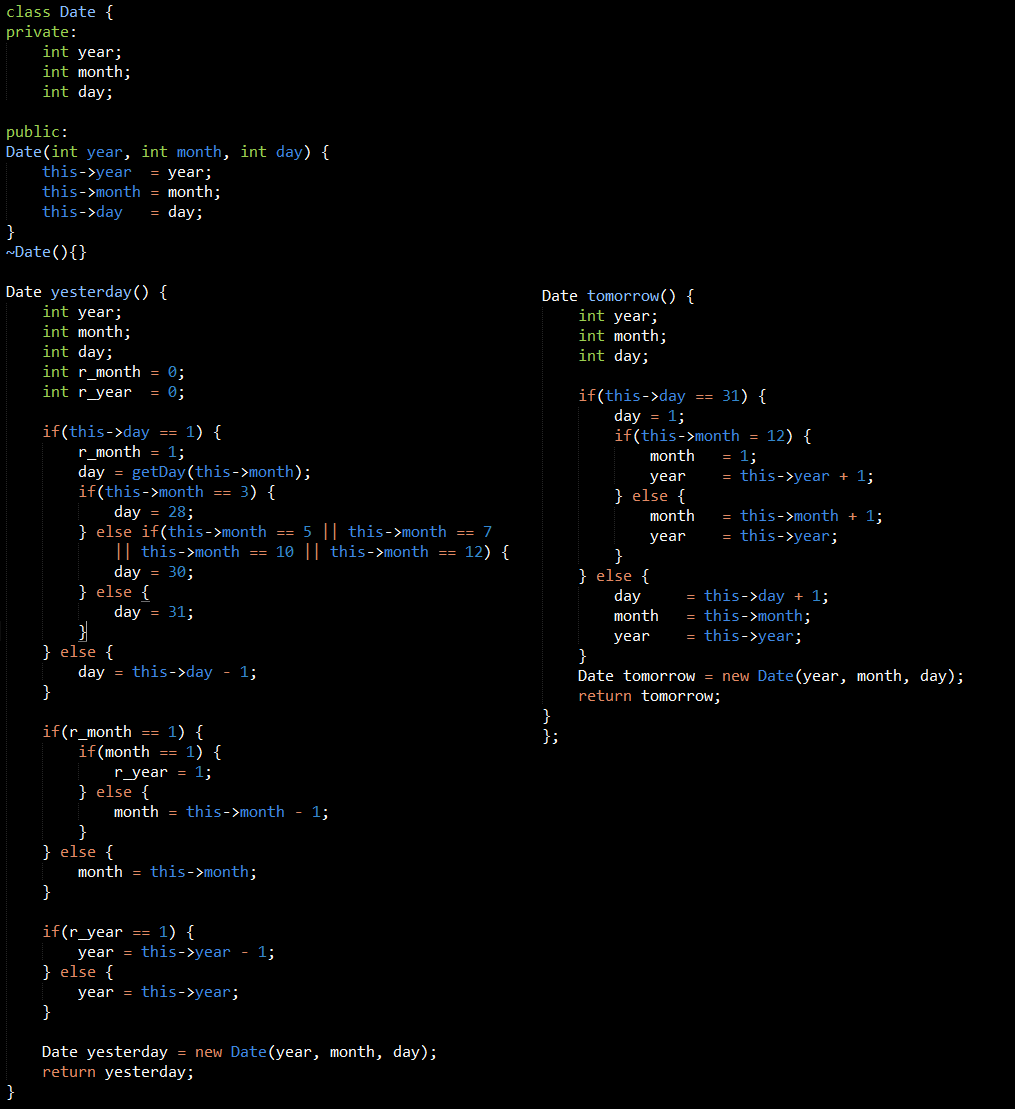
\includegraphics[scale=0.7]{Date.png}\\
Class invariant: \\
$
\begin{tabular}{l | l}
12 \leq \text{month} \leq 1		&	[31, 30, 28]_{\perp\text{month}} \geq \text{day} \geq 1
\end{tabular}
$

\section*{Problem 5.4}
\hspace*{-1 cm}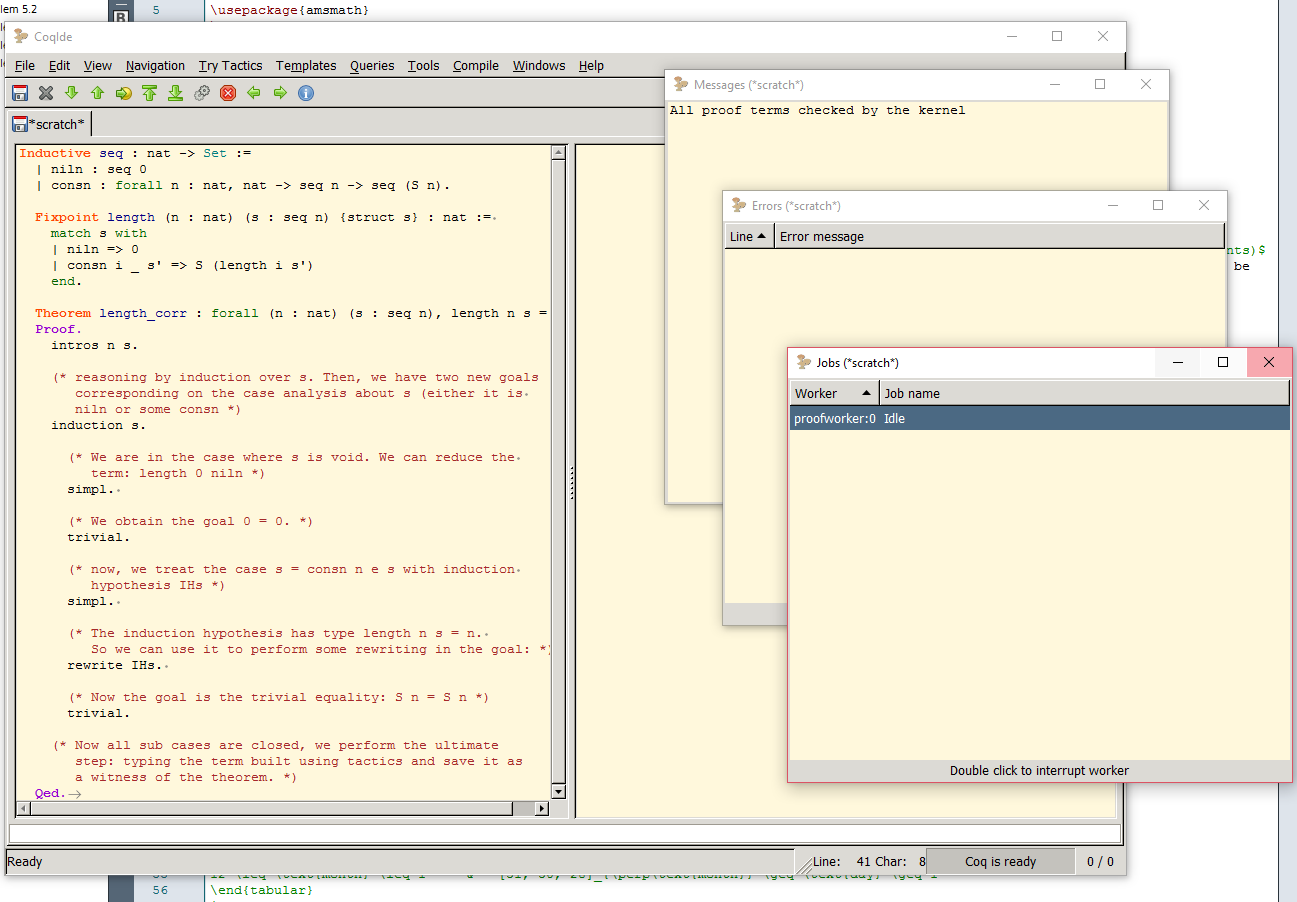
\includegraphics[scale=0.6]{proof_1.png}
\end{document}